% Cheminformatics (4 weeks)

Chemical informatics is the branch of chemistry that attempts to solve chemical problems algorithmically on the computer, such as predicting reactivity based on substructure search or quantum chemical DFT calculations. \emph{RDKit} has become particularly established for this. It is an open-source based cheminformatics toolkit written in C++, but can also be used with Python, Java or JavaScript. Among other things, it includes the following functionalities:

\begin{itemize}
    \item Reading and writing of molecules
    \item Working with molecules in 2D and 3D
    \item Drawing 2D depictions
    \item Substructure search
    \item Chemical transformations
    \item Maximum common substructure
    \item Fingerprints and molecular similarity
    \item Descriptor calculation
    \item Chemical reactions
    \item Chemical features and pharmacophores
\end{itemize}

A central and fundamental area of cheminformatics is the digital \emph{representation of molecules}. For this, we had already introduced graph theory, whereby a molecule can be represented as a graph (vertices are the atoms and edges and their weight are the bonds as well as their bond multiplicity) using an adjacency list or adjacency matrix. Additional information, such as element, stereochemistry, charge or aromaticity, can also be stored in the vertex. The problem with this representation is that it is not very efficient for storage and molecules are difficult to compare. The standard file format for saving chemical structures with coordinates (from crystal structures) is, however, the \emph{Molefile} format, which works with a connection table and is shown below.

\begin{center}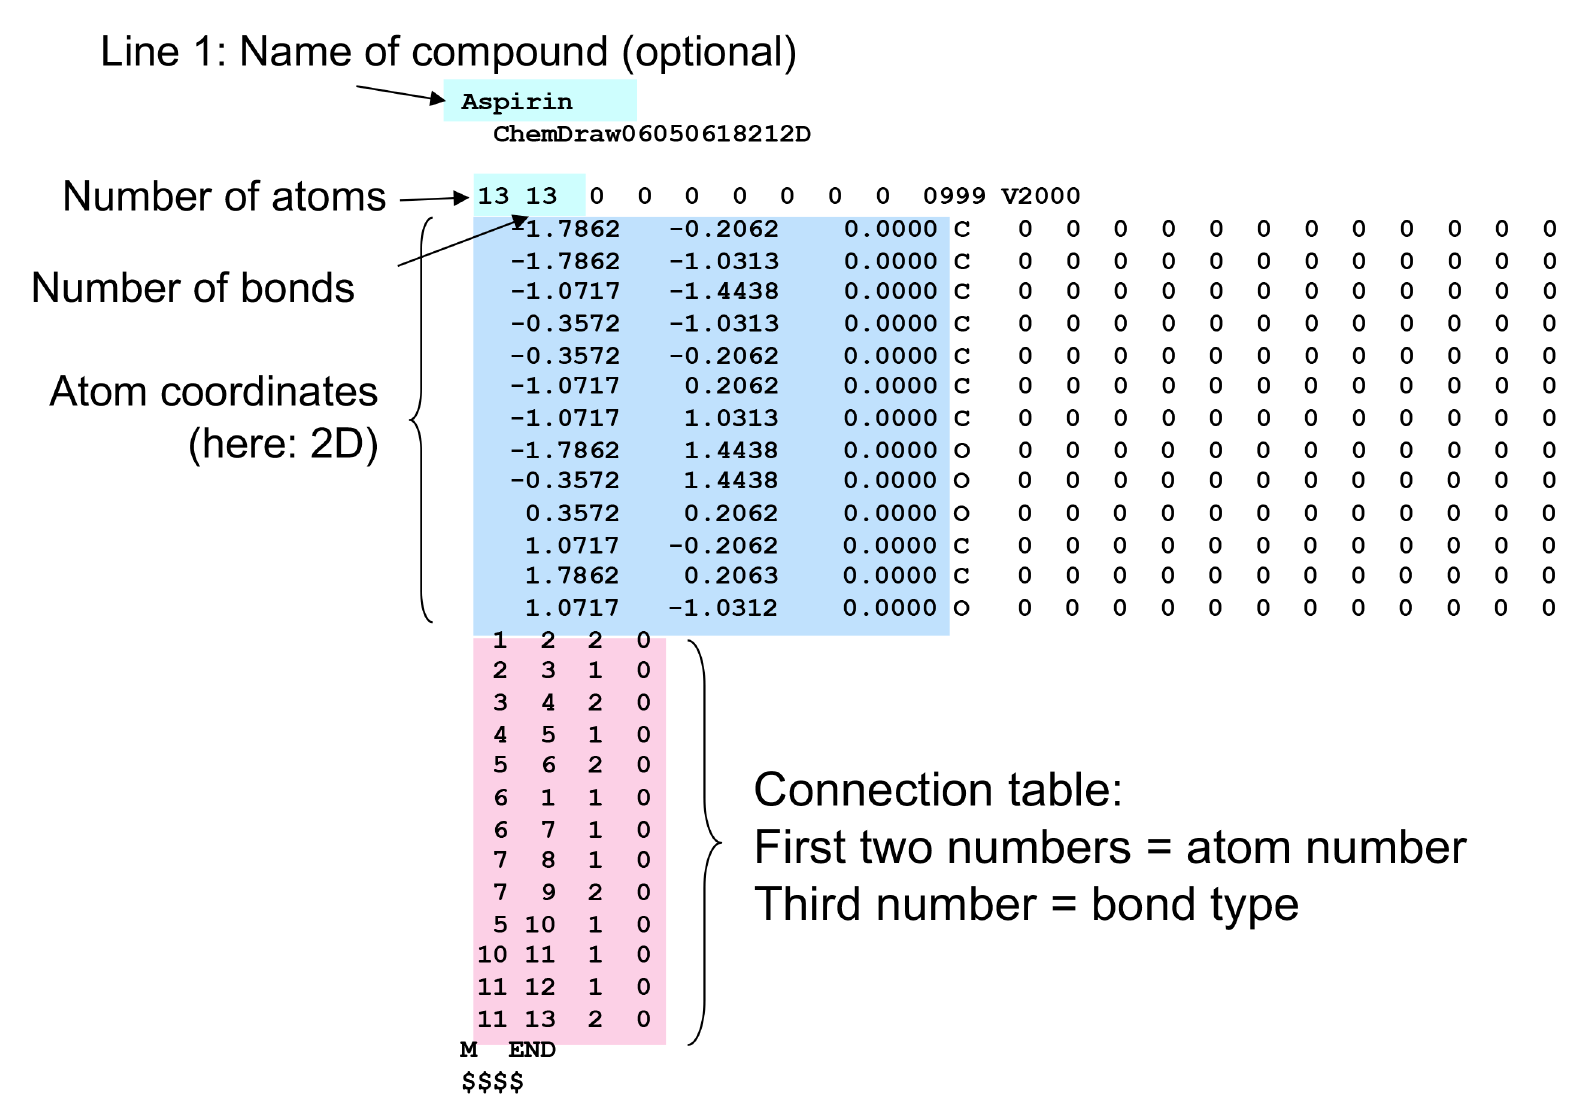
\includegraphics[width=0.70\textwidth]{img/cheminformatics/DataFormat.png}\end{center}

\subsection{1D representation}

The most efficient way to represent molecules for storage is a 1D representation. Furthermore, it can be easily interpreted by a computer and searched in a database. However, it is important that the representation is \emph{reversible}, that the transformations 2D $\rightarrow$ 1D and 1D $\rightarrow$ 2D can be carried out without any problems, and that the representation is \emph{unique}. To achieve this, stereochemistry and aromaticity must be retained in the representation. Examples of such representations are the IUPAC name, WLN, SLN, SMILES and InChI, although we will only deal with the latter two in the following.

\subsubsection{SMILES}

SMILES stands for \emph{Simplified Molecular Input Line Entry System}. It was introduced in 1988 and is based on representing the chemical structure using letters according to established rules. On the computer, a \emph{minimum spanning tree} is first created from a graph, which is then translated into the SMILES using a \emph{depth-first} algorithm, whereby different applicable SMILES are generated depending on which atom is started with. Therefore, a \emph{canonicalization} is needed to make the representation unique. SMILES follows the following rules:

\begin{itemize}
    \item Hydrogens as well as single and aromatic bonds are usually omitted, but can be specified explicitly if desired.
    \item \textbf{Atoms:}
    \begin{itemize}
        \item General: Atomic symbol in square brackets
        \item “Organic” subset (= B, C, N, O, P, S, F, Cl, Br, I) can be written without brackets if the number of attached Hs is “normal”.
        \item Attached hydrogens and formal charges always specified inside brackets.
        \item Atoms in aromatic rings are specified by lower case letters (i.e. c, n).
        \item Stereocentres are specified with @ (anti-clockwise writing of neighbors) and @@ (clockwise writing of neighbors) inside brackets.
    \end{itemize}
    \begin{center}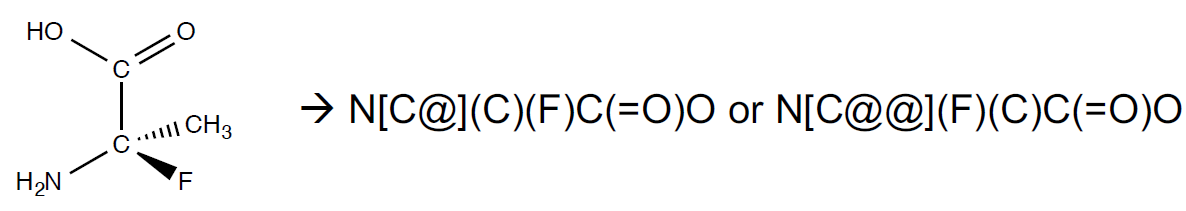
\includegraphics[width=0.65\textwidth]{img/cheminformatics/SmilesRulesAtoms.png}\end{center}
    \item \textbf{Bonds:}
    \begin{itemize}
        \item Single bond: “-”, double bond: “=“, triple bond: "\#" aromatic bond: “:”
        \item Cis/trans double bonds: use of “/” and “$\backslash$”, e.g.
    \end{itemize}
    \begin{center}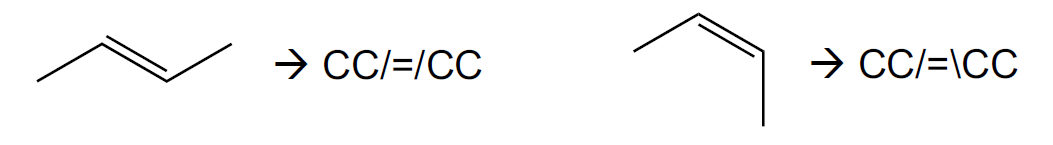
\includegraphics[width=0.65\textwidth]{img/cheminformatics/SmilesRulesBonds.png}\end{center}
    \item \textbf{Branches:}
    \begin{itemize}
        \item Specified by parentheses
        \item Can be nested or stacked
    \end{itemize}
    \begin{center}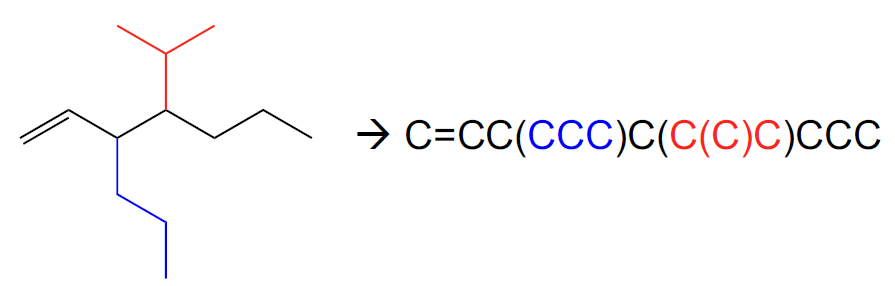
\includegraphics[width=0.65\textwidth]{img/cheminformatics/SmilesRulesBranches.png}\end{center}
    \item \textbf{Cyclic structures:}
    \begin{itemize}
        \item Represented by breaking one bond (to get spanning tree) and numbering the ring-closure atoms
        \item Ring-closure digits can be reused
    \end{itemize}
    \begin{center}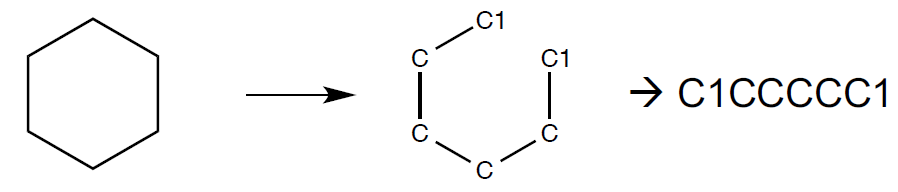
\includegraphics[width=0.65\textwidth]{img/cheminformatics/SmilesRulesCyclic.png}\end{center}
    \item \textbf{Aromaticity}
    \begin{itemize}
        \item Aromaticity in cheminformatics is a concept! Different definitions/algorithms exist (discussed later). Do not confuse it with a physical phenomenon
        \item Aromatic bonds are usually omitted
        \item Atoms in an aromatic ring are specified by lower case letters
    \end{itemize}
    \begin{center}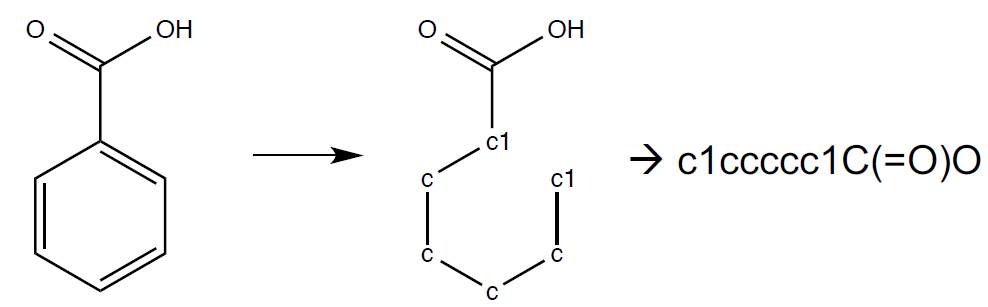
\includegraphics[width=0.65\textwidth]{img/cheminformatics/SmilesRulesAromaticity.png}\end{center}
\end{itemize}

\textcolor{red}{Beispiele aus den slides machen und einfügen.}

% not finished code
%\lstinputlisting[language=C++]{src/cheminformatics/smiles.cpp}

\subsubsection{Canonicalization}

As already mentioned, several correct SMILES can be used for one molecule, depending on which atom you start with. Therefore, a canonicalization must be performed to create a unique and reproducible numbering of the atoms of a molecule.

\deff{Graph Isomorphism}{Two graphs are isomorphic when there is a 1-to-1 mapping (a permutation) from the vertices of one graph to the vertices of the other, such that the edge connections are respected. In short, isomorphic graphs are structurally the same, but the labeling of the vertices is different.}

\deff{Graph Invariant}{In graph theory, a graph property or graph invariant is a property of graphs that depends only on the abstract structure, not on graph representations such as particular labellings or drawings of the graph. Therefore, two isomorphic graphs have the same invariants.}

In the example of cheminformatics, the invariants of a graph are usually a combination of information such as element, number of bonds, number of hydrogens, ring information, etc.

\paragraph{Morgan's Algorithm}
Morgan's algorithm is a canonicalization algorithm for chemical compounds presented in 1965 that uses the number of bonding partners (excluding hydrogen) as invariants. The algorithm proceeds as follows:

\begin{enumerate}
    \item \emph{Step 1: Find invariants}
    \begin{itemize}
        \item First assign the initial invariants to each atom, i.e. the number of bonds.
        \item Then assign new invariants for each atom, which are the sum of the invariants of the neighbors (excluding its own invariant). Repeat this step until the number of invariants no longer increases.
    \end{itemize}
    \begin{center}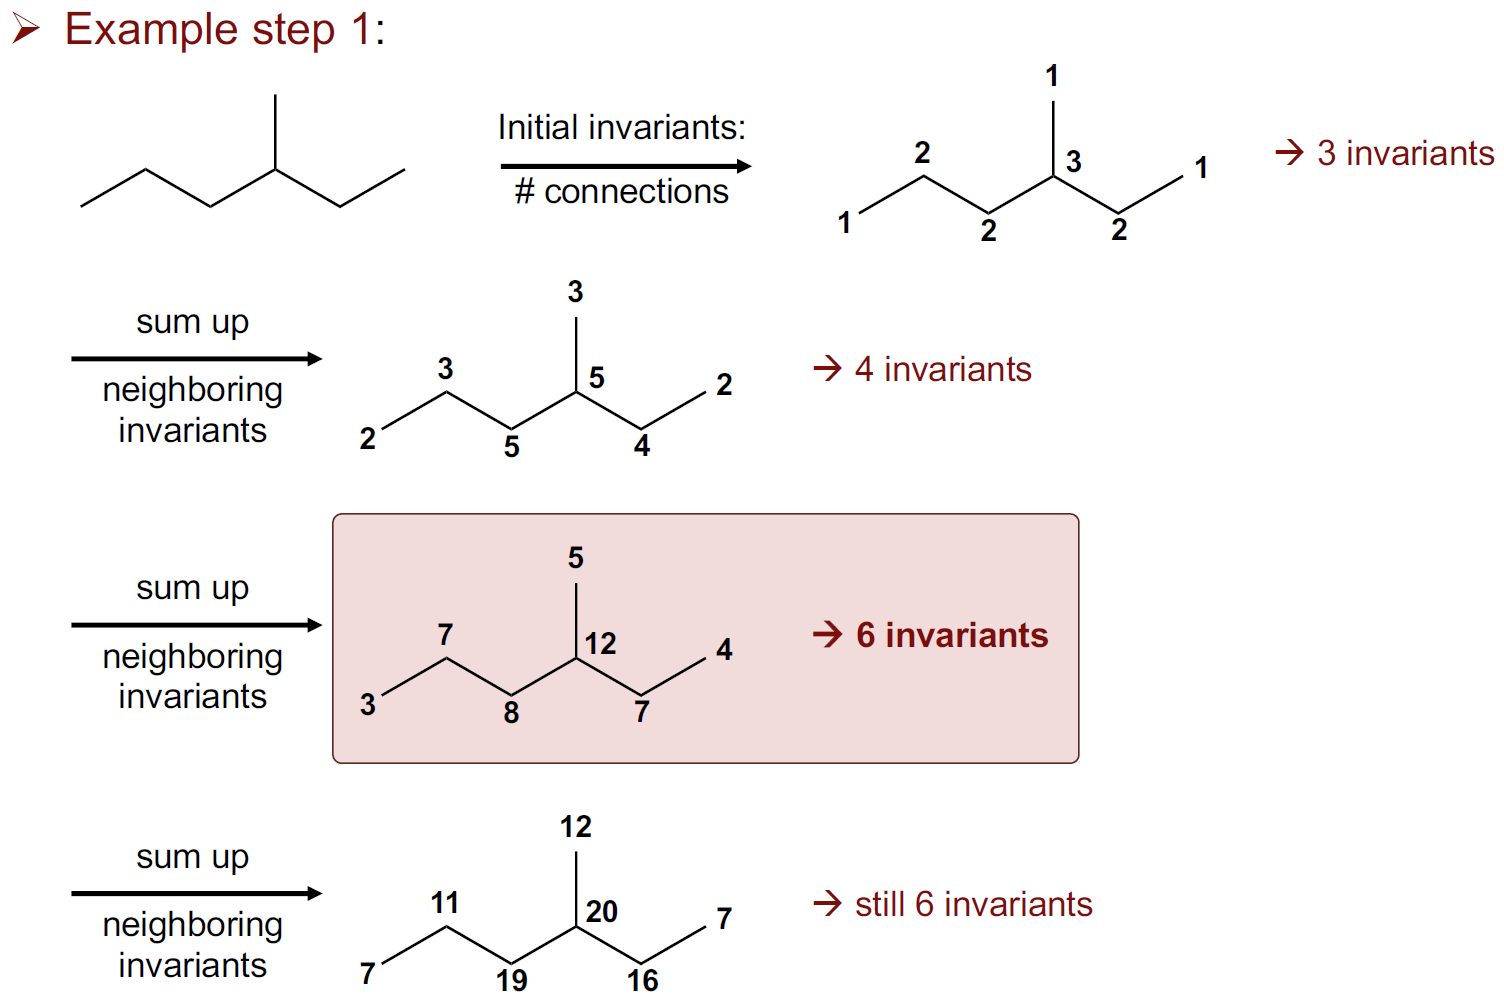
\includegraphics[width=0.85\textwidth]{img/cheminformatics/Morgan1.png}\end{center}
    \item \emph{Step 2: Set ranks}
    \begin{itemize}
        \item Take the graph where the number of invariants increased last time (not the graph where they were increased but the number of invariants remained the same).
        \item Take the largest invariant and set the rank of the atom to 1.
        \item Take the neighbors of the atom with rank 1, order them by descending invariants and give them the ranks 2-4 accordingly (assuming three are bonded).
        \item Now always choose the atom with the smallest rank and assign ranks to its neighbors according to descending invariants. Repeat this step until each atom has a rank.
    \end{itemize}
    \begin{center}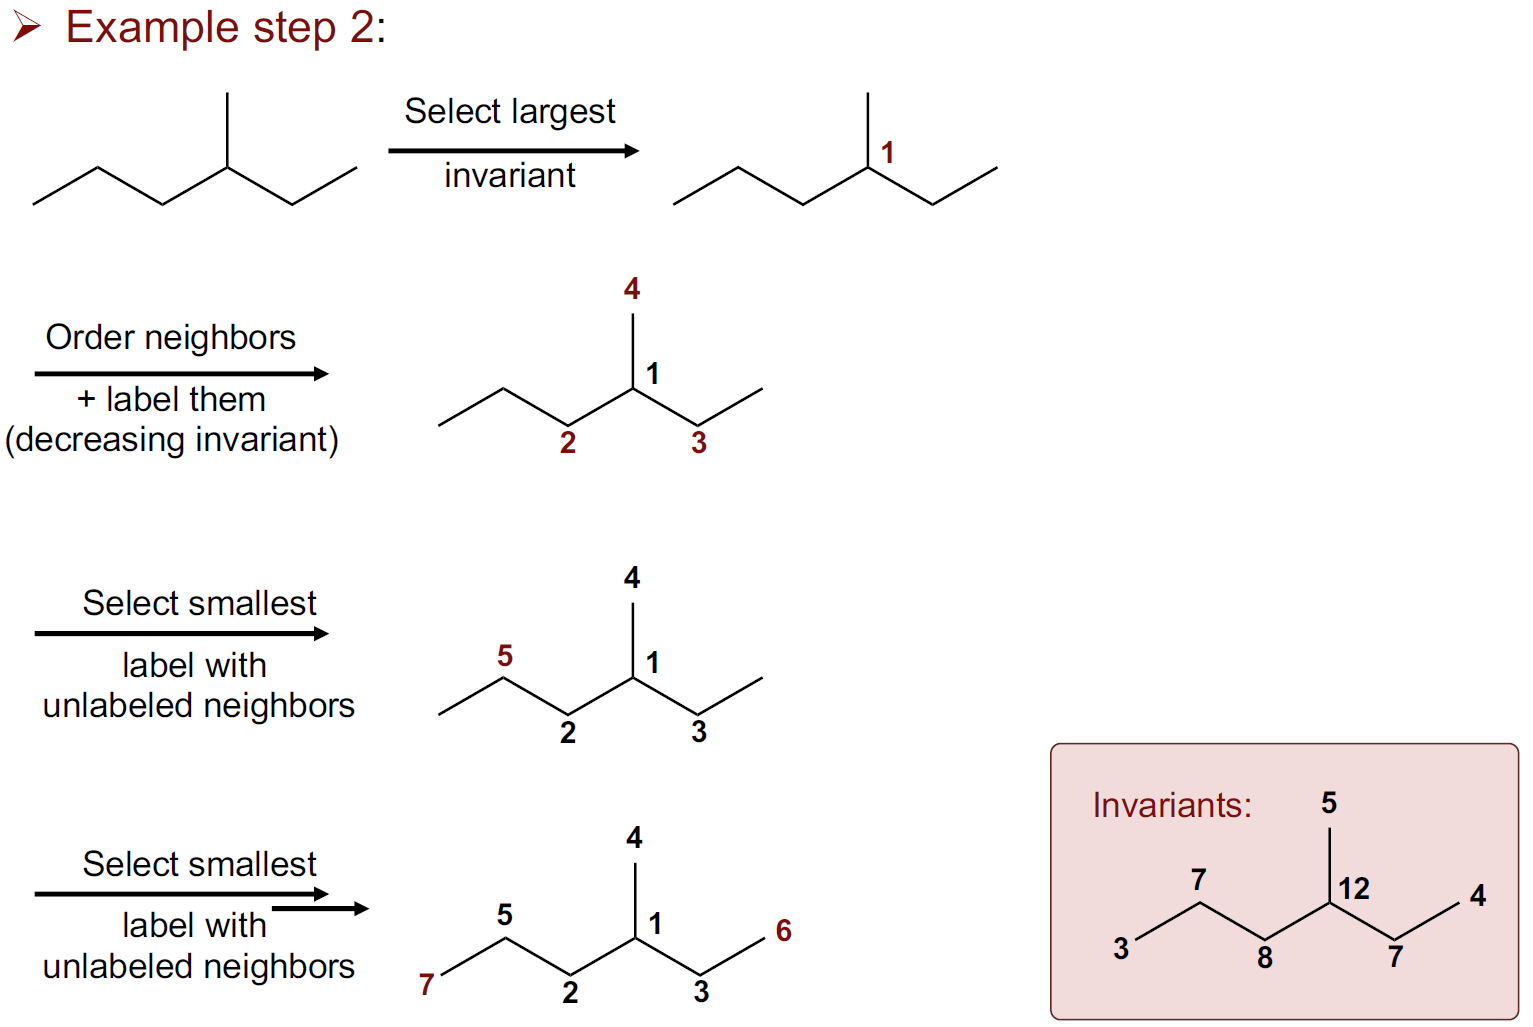
\includegraphics[width=0.85\textwidth]{img/cheminformatics/Morgan2.png}\end{center}
\end{enumerate}

The main criticism of Morgan's algorithm is that the summation step produces ambiguous results, which is why uniqueness cannot be proven. One way to solve this is to also include the atom type and bond multiplicity. Furthermore, oscillations can occur for certain symmetrical molecules, so that the first step has no termination condition.

% not finished code
%\lstinputlisting[language=C++]{src/cheminformatics/morgan.cpp}

\paragraph{Cangen Algorithm}

Just like Morgan's algorithm, CANGEN uses the number of binding partners to find the invariants. However, in the iterative calculation, CANGEN uses the product of primes instead of the sum of the invariants of the neighbors, as in Morgan's algorithm, to minimize ambiguities. However, a unique numbering cannot be proven here either.

\begin{enumerate}
    \item 
\end{enumerate}

% not finished code
%\lstinputlisting[language=C++]{src/cheminformatics/cangen.cpp}

\subsubsection{InChI}

\subsubsection{Ring perception}

The idea behind ring perception is to develop an algorithm that can automatically detect ring structures in 1D representations of molecules. The whole thing must therefore be independent of the projection, orientation and labeling of the ring system.

\begin{itemize}
    \item \textbf{Chords:}
    \begin{itemize}
        \item Minimum number of bonds whose removal is required to turn a structure from cyclic to acyclic.
    \end{itemize}
    \item \textbf{Nullity:}
    \begin{itemize}
        \item Number of chords that can be calculated using the formula below, where components stands for the number of closed graphs (always 1 for a molecule).
    \end{itemize}
    \begin{align}
        \mu=\#_\mathrm{bonds}-\#_\mathrm{atoms}+\#_\mathrm{components}
    \end{align}
    \item \textbf{Cycle:}
    \begin{itemize}
        \item Traversable node by node in a single path back to the start.
    \end{itemize}
\end{itemize}

The size we now want to determine exactly is the smallest set of smallest rings (SSSR), in which as many rings of the smallest possible size as possible are found. 

\begin{center}
    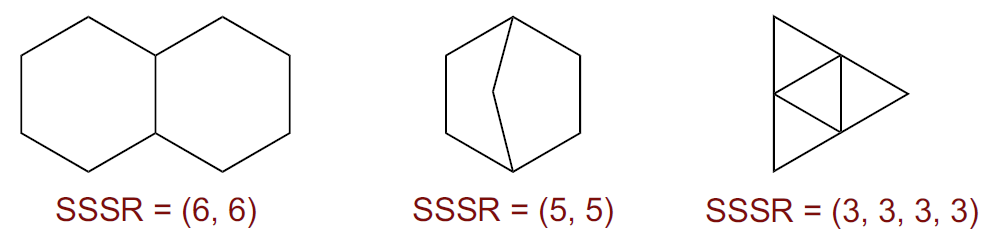
\includegraphics[width=0.85\textwidth]{img/cheminformatics/RingPerceptionSssr.png}
\end{center}

\paragraph{Figueras' algorithm}
Figueras' algorithm is an algorithm presented in 1996 to determine the SSSR of a molecule. The algorithm proceeds as follows:

\begin{enumerate}
    \item 
\end{enumerate}

\begin{center}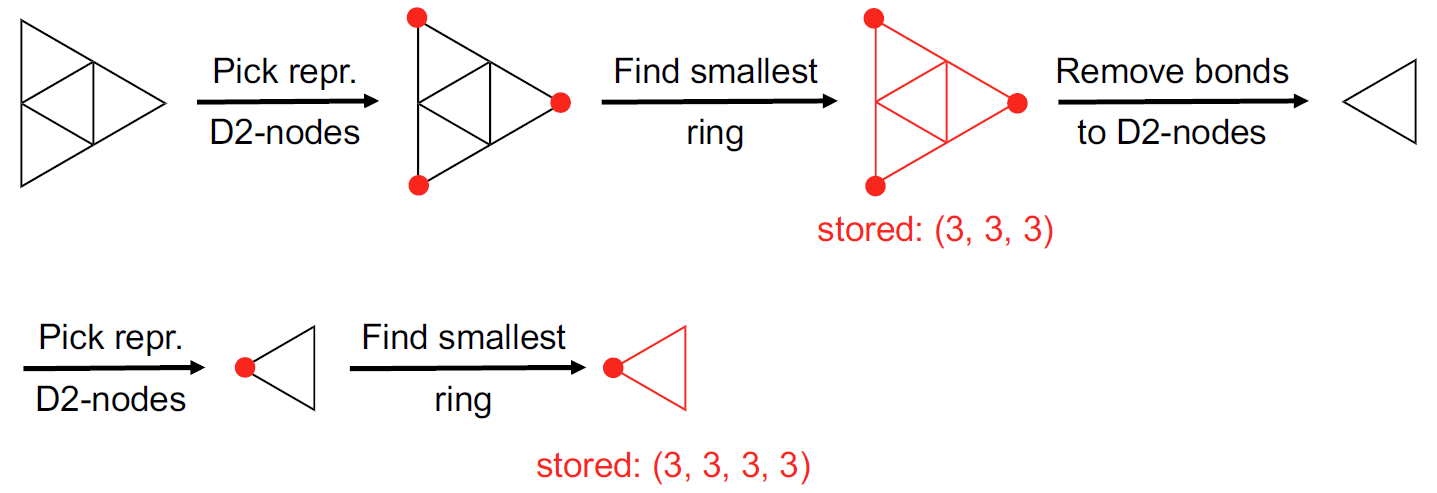
\includegraphics[width=0.85\textwidth]{img/cheminformatics/RingPerceptionFigueras1.png}\\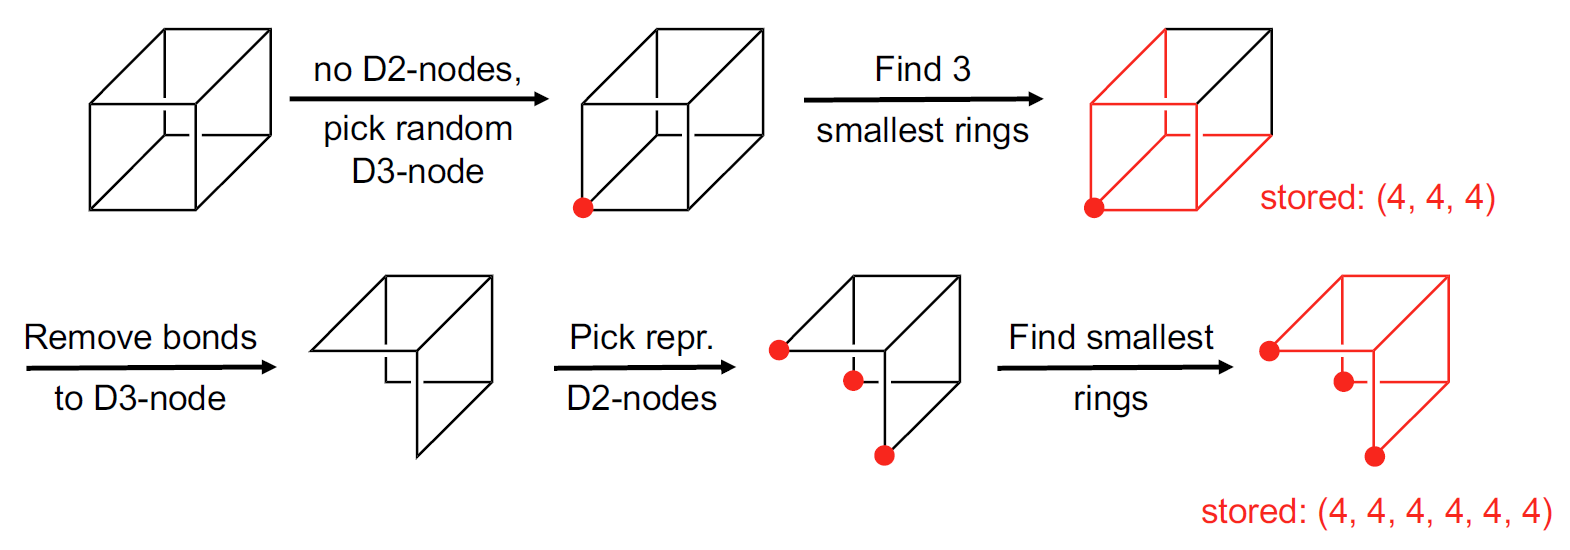
\includegraphics[width=0.85\textwidth]{img/cheminformatics/RingPerceptionFigueras2.png}\end{center}

% not finished code
%\lstinputlisting[language=C++]{src/cheminformatics/figueras.cpp}

\subsubsection{Aromaticity detection}

The definition of armoaticity is not trivial and the implementation in cheminformatics is still under discussion, because for cheminformatics a definition has to be found that is as simple as possible, that applies in most cases and is co-agent with SMILES and substructure search. Therefore, the cheminformatics definition does not necessarily imply physical properties of the molecule.

\begin{itemize}
    \item \textbf{Hückel's rule:}
    \begin{itemize}
        \item $(4n+2)\;\pi$-electrons $\rightarrow$ aromatic
    \end{itemize}
    \item \textbf{Extension of Hückel’s rule:}
    \begin{itemize}
        \item $(4n+2)\;\pi$-electrons and all atoms $\mathrm{sp}^2$ (planar) $\rightarrow$ aromatic
    \end{itemize}
\end{itemize}

With SMILES, both the Kekulè form (localized double bonds) can be used, as well as the explicit labeling of aromaticity with lowercase letters, whereby the latter is the preferred output of SMILES, since the former creates an artificial asymmetry.

\begin{align*}
    &\textit{Exapmle: benzene}&\begin{cases}
        \textit{Kekulè: }&\text{C1=CC=CC=C1}\\
        \textit{SMILES: }&\text{c1ccccc1}
    \end{cases}
\end{align*}

Aromatic systems over several rings are generally more difficult. For example, non-aromatic single bonds between two aromatic rings should be explicitly written with “-” in SMILES (e.g. biphenyl with c1ccccc1-c2ccccc2).

\paragraph{Aromaticity in the RDKit:}
The RDKit uses the Hückel rule for aromaticity, whereby a ring or condensed ring system with $(4n+2)\;\pi$-electrons is considered aromatic. Both bonds and atoms can be aromatic, whereby an aromatic bond must be between two aromatic atoms, but a bond between two aromatic atoms does not necessarily have to be aromatic. This is why in condensed ring systems the individual cycle can be not aromatic, but the overall system is.

\begin{center}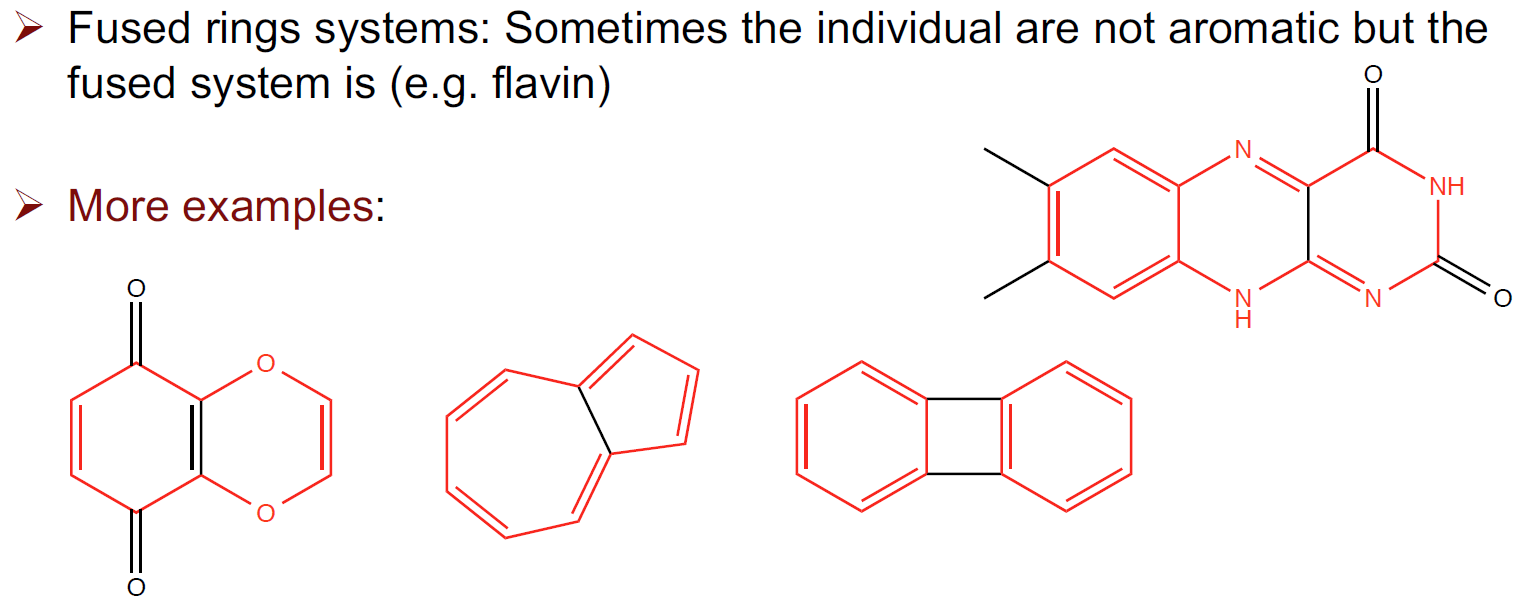
\includegraphics[width=0.85\textwidth]{img/cheminformatics/AromaticRdkit.png}\end{center}

\subsection{Substructure search}

In cheminformatics, a distinction is made between three shifting structure searches:

\begin{itemize}
    \item \textbf{Full structure search:}
    \begin{itemize}
        \item Question: Is this molecule in my database?
        \item Input: Full chemical structure (e.g. SMILES)
        \item Solution: Comparison of SMILES, InChi (keys), internal index number, etc.
    \end{itemize}
    \item \textbf{Substructure search:}
    \begin{itemize}
        \item Question: Does this substructure exist in any molecule of my database?
        \item Input: Query pattern of atoms and bonds (e.g. SMARTS).
        \item Solution: Brute-force, backtracking, partitioning and relaxation
    \end{itemize}
    \item \textbf{Superstructure search:}
    \begin{itemize}
        \item Question: Are any molecules in my database substructures of the query?
        \item Input: full chemical structure (e.g. SMILES)
        \item Solution: same as substructure search
    \end{itemize}
\end{itemize}

\subsubsection{SMARTS}

SMARTS (SMILES arbitrary target specification) is an extension of the classic SMILES to describe molecular patterns (substructures). With SMILES only exact atoms can be specified, whereas with SMARTS wildcards for atoms and bonds are possible, which can simplify the substructure search.

\begin{itemize}
    \item \emph{Atoms:}
    \begin{itemize}
        \item Specified by either element symbol or number: e.g. [#6] à any carbon
        \item “*” : wild card
        \item “A” : any aliphatic atom
        \item “a” : any aromatic atom
        \item “D” followed by a number : degree (number of explicit connections)
        \item “R” followed by a number n : in n smallest rings
        \item “r” followed by a number n : in a smallest ring of size n
        \item “H” followed by a number : number of adjacent hydrogens
        \item H has now two meanings: e.g. [H] $\rightarrow$ hydrogen atom, [*H2] $\rightarrow$ any atom with two hydrogens
        \item Multiple possible matches are separated by a comma: e.g. [C,N] $\rightarrow$ either aliphatic C or N
    \end{itemize}
    \item \emph{Bonds:}
    \begin{itemize}
        \item “\~” : any bond
        \item “@” : any ring bond
    \end{itemize}
    \item \emph{Logical operators:} combinations of atom and bond specifications
    \begin{itemize}
        \item “!” : NOT, e.g. [!C] à not aliphatic carbon
        \item “\&” : AND (high priority)
        \item “,” : OR
        \item “;” : AND (low priority)
        \item Operator priority: “!” > “&” > “,” > “;”
    \end{itemize}
    \item \emph{Aromaticity:}
    \begin{itemize}
        \item Note: a double bond is not matched to an aromatic bond!
    \end{itemize}
\end{itemize}

\begin{center}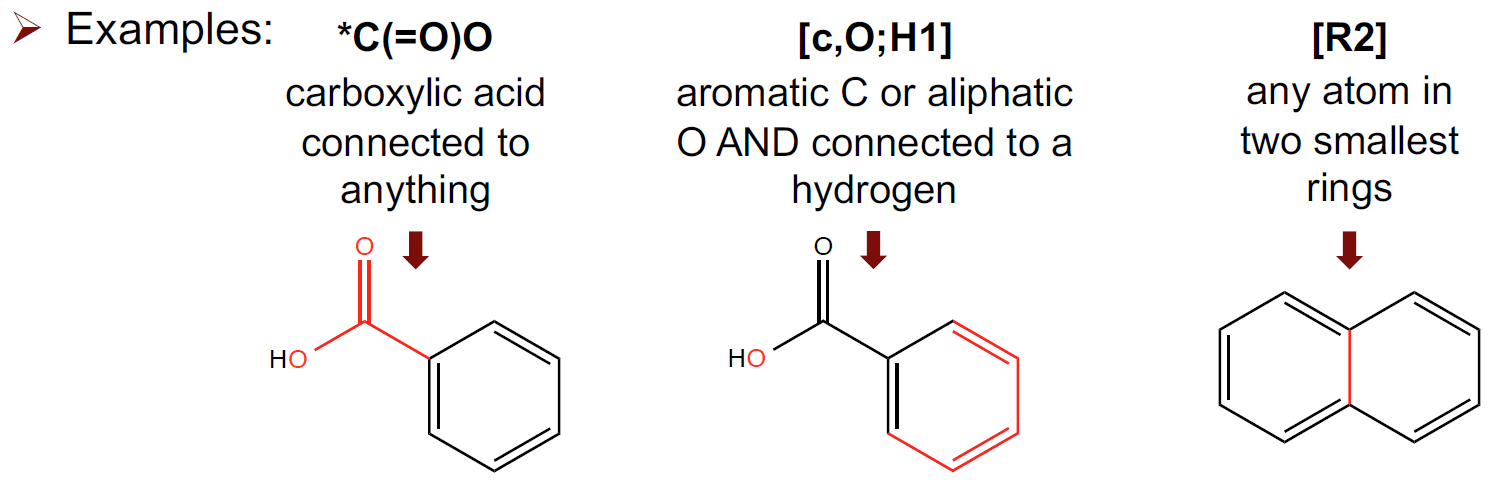
\includegraphics[width=0.85\textwidth]{img/cheminformatics/SubstructureSmartsExample.png}\end{center}

\subsubsection{Subgraph isomorphism}

\subsection{Chemical reactions}

\subsection{Dimensionality reduction}

\subsection{Fingerprints}

\subsection{Maximum common substructure}

\subsection{Scaffolds}

\subsection{Generation of 3D coordinates}

\subsubsection{Distance geometry}

\subsection{Clustering}

\subsubsection{Hierarchical}

\subsubsection{Application to chemical space}

\subsubsection{Non-hierarchical}

\subsubsection{Application to conformations}